\chapter{Introduction}
This chapter introduces the basic idea of interaction between CFS++
and a scripting language (here: Tcl).

\section{Scripting within CFS++}
CFS++ offers the possibility to extend the static definition of
parameters within the xml-file dynamically during program execution by
using the {\em Tcl scripting language}. Therefore it creates a local
Tcl interpreter and extends it with functions to interact with CFS++.
This enables one to combine the
Tcl-inerhent functions (string manipulation, file-IO, mathematical
expression) together with some additional functions offered by CFS
(Grid handling, set/get boundary conditions/results, debugging).
\newline

\noindent
Some example scenarios might be as follows:
\begin{itemize}
\item{\bf Result-driven Feedback}: By coupling the calculated values of a
  physical problem to its boundary conditions / load values one can
  realize control mechanism like feed-back control or dynamic loading.
\item {\bf Interfacing to external programs}: The ability to get and
  set values in each step and to call external programs allows one to
  interface with almost arbitrary programs. One could include for
  example matlab or an external circuit simulator to interact with CFS.
\item {\bf Complex Boundary / Load Conditions}: Using the methods of
  the grid class it is possible to easily prescribe space-dependent
  boundary conditions or to load values from external text files.
\item {\bf Debugging / Information}: Additional information,
  e.g. element matrices or vector norms, can be retrieved dynamically
  without re-compiling the program or using an external debugger.
\end{itemize}

To activate scripting within CFS++, it has to be called as follows:
\begin{verbatim}
cfs -e=example.tcl problemFile
\end{verbatim}

This triggers the following:
\begin{enumerate}
\item CFS creates a local Tcl interpreter with additional methods for
  interaction 
\item The tcl-file gets parsed and evaluated.
\item At certain points in the program pre-defined event procedures
  are called, where the script commands are executed.
\end{enumerate}
The general program flow involving scripting can be seen in Fig. \ref{fig:progFLow}.
\begin{figure}[H]
 \begin{center}
    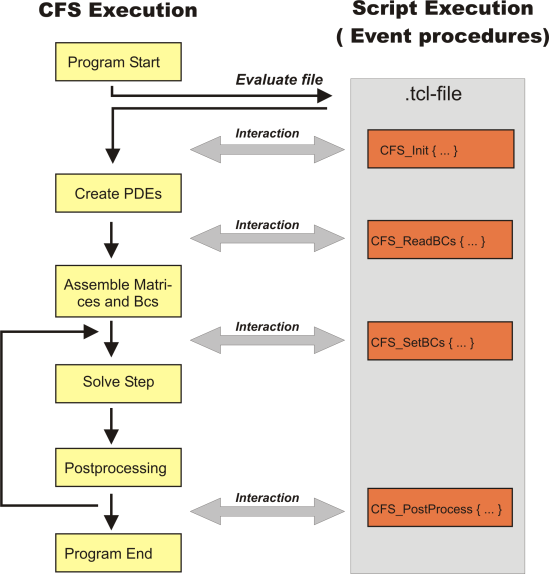
\includegraphics[width=16cm]{pics/program-flow}
    \caption{Program flow of CFS++ with scripting}
        \label{fig:progFLow}
  \end{center}
\end{figure}

\section{The Tool Command Language (Tcl) }
The only language currently supported is the {\em Tool Command
  Language (Tcl)}. It is a command-oriented simple language, created
by John Osterhout. The original purpose was to make communication
between different programs easier, to form more powerful programs.
Some important features about Tcl:
\begin{itemize}
\item Dynamically interpreted language
\item Simple syntactic rules
\item Everything can be referred to as string
\item Powerful datatypes like Hashes and Lists
\item Platform independency
\item Easy GUI creation by using {\em TK}
\end{itemize}

More information can be found on \url{http://www.tcl.tk}. 